\chapter{绪论}

\section{研究背景与意义}

随着5G通信与流媒体业务的发展，视频数据已成为网络传输中的主要负载之一。在实时视频通话、云游戏、远程办公与AR/VR等场景中，系统既要控制端到端时延，又要在有限带宽下维持可接受的视觉质量。现有视频编码标准各有取舍：H.264/AVC\cite{ref33-wiegand2003avc}兼容性最好，但在高清和低带宽场景下压缩效率不足；H.265/HEVC在同等画质下可较H.264节省约50\%码率，但专利和授权问题影响了其进一步普及\cite{ref10-sullivan2012hevc}；H.266/VVC具有更高率失真性能\cite{ref1-bross2021vvc}，但编码复杂度和时延更高；AV1\cite{ref61-chen2020av1}提供了开放免版税路径，但硬件生态覆盖仍在完善。

与此同时，以Ballé等人\cite{ref53-balle2017end2end}与Minnen等人\cite{ref54-minnen2018hyperprior}为代表的端到端深度学习编码方案虽然性能卓越，但受限于巨大的算力开销和功耗，难以在边缘设备上部署\cite{ref8-lu2019dvc}。此外，现有深度学习编码工具多针对传统编码框架的局部模块进行优化，缺乏对整体编码过程的感知，通常需要多阶段迭代训练以获得性能提升\cite{ref16-ding2021advances}。

图~\ref{fig:background-blocking}以NVENC硬件编码器在QP=45低码率工况下的重建帧为例，直观展示了上述画质问题：平坦水面区域出现可见的块状纹理（块效应），礁石边缘处亦伴随振铃与细节模糊。这正是本文所要解决的核心工程问题。右侧为本文方案（RAPNet前处理后编码）的重建结果，可以看到相同QP下感知质量已有明显改善。

\begin{figure}[!htbp]
  \centering
  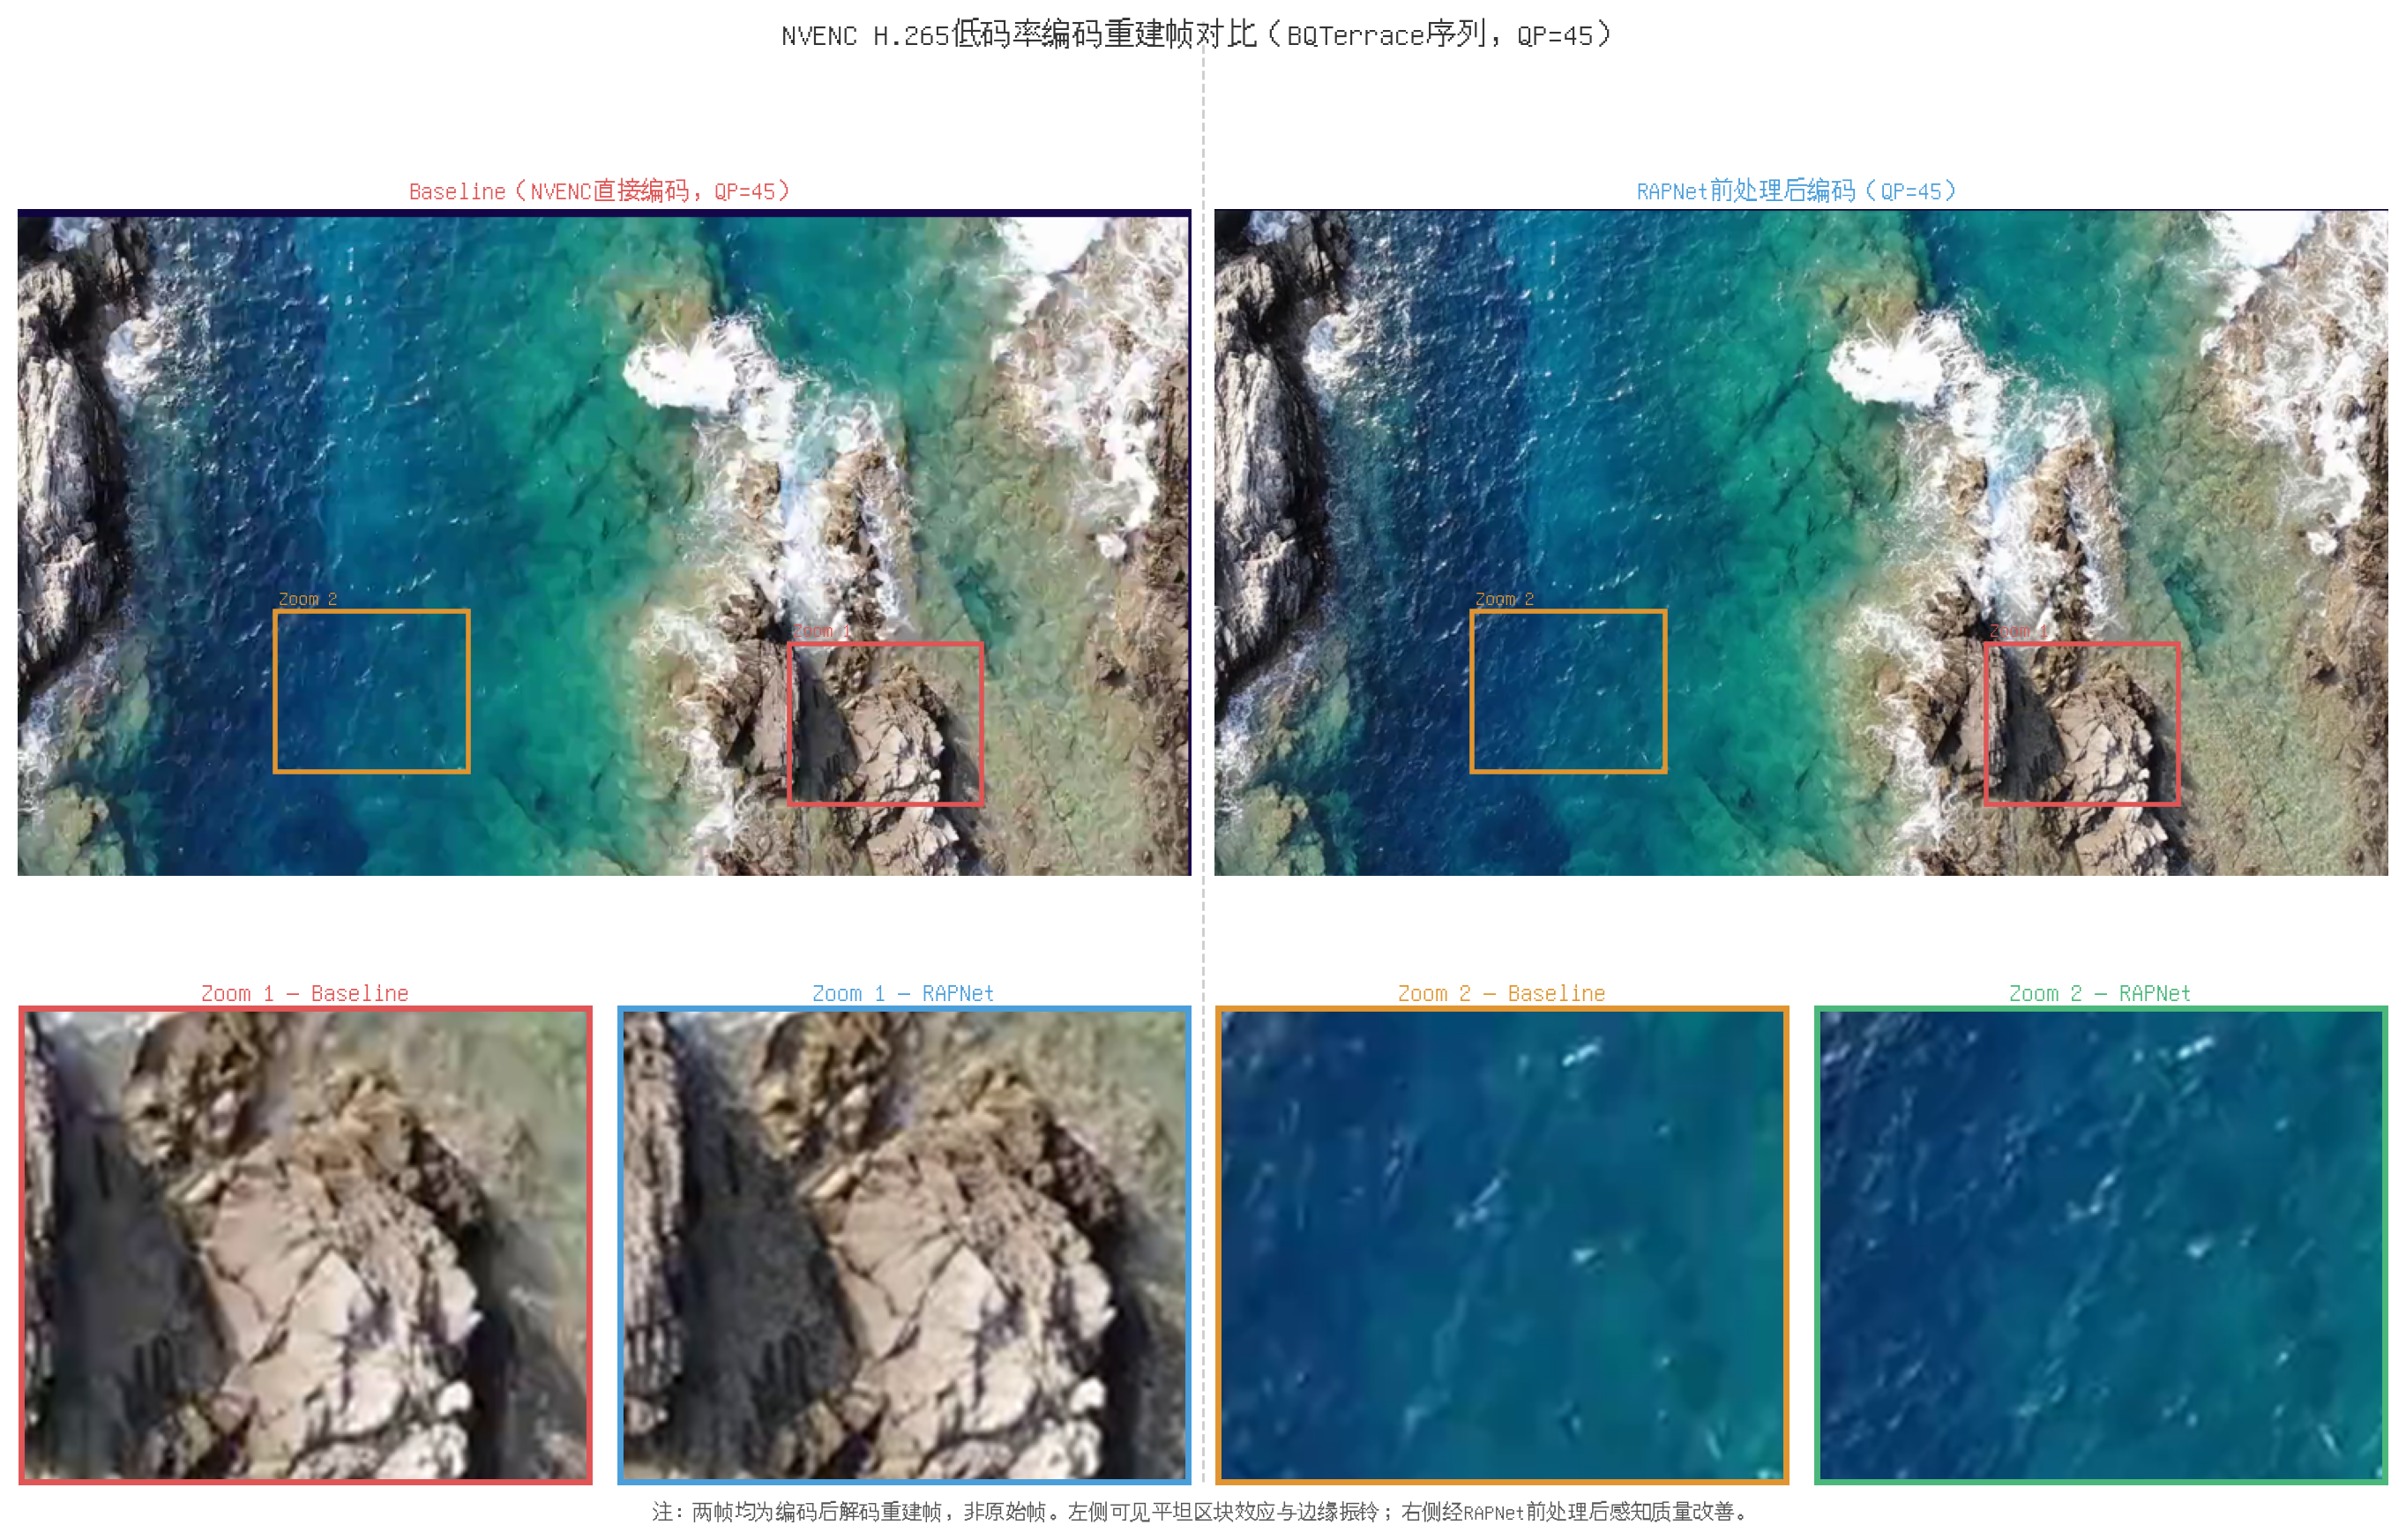
\includegraphics[width=\textwidth]{data/主观图片/background_blocking_comparison.png}
  \caption{NVENC H.265低码率编码重建帧对比（QP=45；两帧均为编码后解码重建帧）}
  \label{fig:background-blocking}
\end{figure}

针对低码率下的画质退化，已有研究提出了超分辨率、去噪和压缩伪影去除等深度增强模型，但这类模型直接用于实时编码仍存在困难。传统滤波方法可以减少部分高频噪声和码率开销，却容易造成过度平滑；基于Transformer的视频复原模型\cite{ref22-liang2022vrt,ref23-liang2022rvrt}虽然在公开数据集上表现较好，但参数量和推理耗时通常难以满足实时编码约束。陈彤等人在综述\cite{ref29-tong2025annual}中也指出，智能编码研究需要同时考虑率失真性能、计算复杂度、跨平台部署和低延迟要求。基于这一背景，本文将研究重点放在编码前处理环节，使模型在进入硬件编码器之前调整输入信号，而不是在解码后再进行离线修复。

相关的深度学习视频编码综述\cite{ref16-ding2021advances}明确指出，前处理的核心目标是在进入标准编码器之前，通过神经网络去除心理视觉冗余\footnote{心理视觉冗余（Psychovisual redundancy）是指人眼视觉系统(HVS)关注不到或不敏感的图像纹理和细节，将其滤除能在不影响主观感受的前提下大幅节省码率开销。}。这也是近年工业界优化编码管道的重要实践，正如bilibili团队\cite{ref17-ma2023rateperception}在RPP方案中所采取的策略：通过利用神经网络将对主观视觉影响较小、且编码开销极大的非本质高频信息\footnote{在视频编码语境中，此处的高频信息通常指人眼视觉系统不敏感的高频纹理或噪声干扰。适度滤除它们能够大幅减少残差能量，进而提升编码效率，同时基本不影响主观感受。}过滤为零，能够直接从源头减少残差能量，进而改善后续硬件编码器的熵编码效率。
    
基于上述问题，本文研究一种面向NVENC低码率视频编码的强化学习前处理方法。该方法不修改硬件编码器内部结构，而是在编码前引入强化学习前处理网络，将NVENC视为黑盒环境，并用真实编码反馈更新前处理策略。在本文实验设置下，系统以5个1080p测试序列为源数据，通过Random Crop构造$960\times540$编码clip；模型参数量为113K，平均前处理时延为5.4ms/帧，并取得平均$-9.48\%$的BD-LPIPS收益。

\section{国内外研究现状}

过去三十余年，主流视频编码技术路线始终围绕变换、预测、环路滤波等规则驱动的模块化工具展开精细化设计与协同优化，并依托MPEG、AVS、AOM等标准化组织构建起成熟的生态体系\cite{ref1-bross2021vvc}。尽管H.266/VVC等新一代标准的压缩效率持续提升，但在工业界大规模商用场景中，受限于极高的计算复杂度、编码时延以及复杂的专利布局，H.264/AVC与H.265/HEVC仍占据着绝对主导地位。

近十年来，随着深度神经网络的快速发展，视频编码领域迎来了新的变革\cite{ref16-ding2021advances}。当前研究已逐渐分化为两条路线：一条是全AI端到端架构，通过深度网络完全替代传统流程\cite{ref8-lu2019dvc,ref6-li2021deep,ref4-cong2025adaptive}，虽然在多个公开数据集上展现出优于H.265/HEVC的压缩效率\cite{ref10-sullivan2012hevc}，但其庞大的算力开销使其难以在边缘设备上部署；另一条是围绕固定硬件编码器进行前后处理协同的AI增强架构\cite{ref9-shen2011downsampling,ref11-vanam2023spie,ref12-vanam2023dcc}，在针对超分辨率\cite{ref2-chan2021basicvsr}、滤波去噪\cite{ref7-lin2019improved}、变换\cite{ref3-chen2018rl}、帧内帧间预测\cite{ref20-chen2023fastmfqe}等环节进行模块化替换或辅助增强。近期也有工作尝试将视频编解码器重新抽象为更通用的张量压缩基础设施\cite{ref18-xu2025llm265}，说明编码技术与AI系统之间的边界正在进一步模糊。后一条路线因其部署灵活、兼容H.26x标准的优势，成为当前工业界与学术界的研究热点。



\section{研究内容与主要工作}

本文提出了由硬件编码器、轻量前处理与AI后处理构成的视频编码增强框架。为突出研究对象与技术主线，本文聚焦于NVENC硬件编码链路中的前处理优化问题，重点研究前处理网络设计、强化学习训练机制及其对率失真性能的影响；后处理联合优化仅作为整体系统背景，不在本文中重点展开。基于上述范围界定，本文的主要工作包括：

\begin{enumerate}
  \item \textbf{课题研究与方案设计}：调研分析H.265硬件编码(NVENC)相较于软件编码的优劣势，特别是其在低功耗、高效率方面的特点以及可能存在的率失真性能损失问题。研究硬件编码结合轻量前处理的视频编码落地路径，设计一套兼顾低功耗和率失真性能的混合编码框架；
  \item \textbf{系统实现与模型构建}：搭建实验系统，集成NVENC硬件编码器，实现基于强化学习的RAPNet\cite{ref27-zhao2025rapnet}前处理算法，AI算法的模型参数量控制在1M以内；
  \item \textbf{实验验证与性能评估}：使用HEVC CTC Class B中的1080p分辨率、YUV420格式标准测试序列\cite{ref-bossen2013ctc}作为源数据，在训练与评测阶段随机裁剪$960\times540$区域构造编码clip，并在CQP模式下以QP$\in\{37,40,42,45,47\}$五个测试点进行量化验证，对比BD-LPIPS感知率失真收益、主观视觉效果、计算复杂度等指标。
\end{enumerate}

\section{本文创新点}

% 论文创新点

本文的主要创新点如下：

\begin{enumerate}
  \item \textbf{编码器感知的强化学习前处理框架}。针对NVENC等硬件编码器"不可导"的固有限制，本文提出将其作为强化学习中的"黑盒环境"纳入优化回路。通过Actor-Critic架构，系统以NVENC编码后的实际码率和感知质量（LPIPS）作为奖励信号，使前处理网络RAPNet能够在不依赖编码器梯度的前提下，自适应地学习针对硬件编码器特性的预补偿策略，有效缓解了低码率场景下的质量崩塌问题。

  \item \textbf{基于Random Crop的高频保持训练策略}。区别于传统的下采样训练方式（如2$\times$下采样到540p），本文采用从1080p原始帧中随机裁剪540$\times$960区域的训练策略。该策略在保持与下采样方案相同计算开销的前提下，完整保留了原始视频的高频纹理和边缘细节，避免了下采样导致的信息丢失，使模型能够学习到更精细的增强策略。

  \item \textbf{频域感知的复合损失函数设计}。除策略梯度损失外，本文设计了一套基于空间频率分解的辅助损失体系：（1）低频结构保持损失（通过$5 \times 5$均值滤波约束低频内容一致性）；（2）非边缘区域高频抑制损失（利用Sobel边缘检测生成软掩模，仅在平坦区域惩罚高频修改，避免边缘模糊）；（3）边缘聚焦损失（鼓励模型将修改集中在边缘区域，提升主观锐度）。该设计使模型在提升编码效率的同时保持了视觉自然度。
\end{enumerate}

\section{论文结构安排}

本文共分为五章，各章内容安排如下：

第一章为绪论，介绍研究背景与意义、国内外研究现状概述、研究内容与主要工作、本文创新点以及论文结构安排。

第二章为相关工作与理论基础，系统梳理视频编码标准演进、编码器感知前处理技术发展脉络、后处理技术分析以及强化学习基础理论，并结合模型复杂度与性能分析，明确本文的技术选型依据。

第三章详细阐述系统设计与实现，包括基于Actor-Critic架构的视频前处理优化系统的整体设计、状态空间与动作空间的定义、复合奖励函数设计及网络损失函数建模。

第四章进行实验与结果分析，在多个QP测试点上对比基线编码与集成增强前处理，从BD-LPIPS、主观视觉效果、计算复杂度等维度验证方案；同时分析近50个强化学习训练版本，总结通道崩塌、梯度爆炸等失败案例及工程处理方法。

第五章总结全文，分析方案局限，并展望端到端联合优化等后续工作。
